\documentclass[a4paper]{article}

\usepackage[utf8]{inputenc}
\usepackage[english]{babel}
\usepackage{graphics}
\usepackage{caption}
\usepackage{subcaption}
\usepackage[demo]{graphicx}
\usepackage{enumitem}
\usepackage{longtable}
\usepackage{listings}
\usepackage{listingsutf8}
\usepackage{framed}
\usepackage{float}
\usepackage{hyperref}
\usepackage{amsmath}

\begin{document}

\begin{titlepage}

\begin{center}
\vspace*{-1in}
\begin{figure}[htb]
\begin{center}

\includegraphics[width=8cm]{logoUZ.png}
\end{center}
\end{figure}

\vspace*{0.3in}

UNIVERSIDAD DE ZARAGOZA \\

\vspace*{0.3in}

\begin{large}
SISTEMAS Y TECNOLOGÍAS WEB\\
\end{large}
\vspace*{0.2in}
\begin{Large}
\textbf{FelinoTweets} \\
\end{Large}
\vspace*{0.3in}
\begin{large}
\end{large}
\vspace*{0.5in}
\rule{80mm}{0.1mm}\\
\vspace*{0.1in}
\begin{large}
Autores: \\
Alejandro Márquez Ferrer (NIP: 566400)\\
Jaime Ruiz-Borau Vizárraga (NIP: 546751)\\
Alejandro Royo Amondarain (NIP: 560285)\\

\end{large}
\end{center}

\end{titlepage}
\tableofcontents

\newpage
\section{Resumen}

	\paragraph{} El trabajo propuesto tiene como objetivo el desarrollo de un sistema que permita gestionar, mediante una interfaz típica de control de acceso de usuarios, una o varias cuentas de \textit{Twitter}.

\section{Propuestas similares - Hootsuite}

	\paragraph{} Se ha analizado principalmente un servicio web similar a la propuesta, \textit{Hootsuite}. Esta herramienta ofrece en su vista principal un panel de control (\textit{dashboard}) para gestionar las cuentas de diferentes redes sociales (\textit{Twitter}, \textit{Facebook}...). Es posible añadir nuevas columnas o eliminarlas para estar al tanto de la mayor cantidad de información posible. 
	
	\paragraph{} Se proporcionan varias versiones de esta aplicación, una gratuita (con funcionalidades limitadas) y otra de pago que ofrece al usuario servicios adicionales como el de realizar informes de estadísticas sobre sus redes sociales.

\section{Arquitectura de alto nivel}
	\paragraph{} A continuación se presenta un diagrama arquitectural de alto nivel con la estructura de la aplicación desarrollada, seguido de una descripción más en detalle de cada una de las partes que la componen:
	\begin{figure}[H]
		\centering
		\includegraphics[width=260px]{diagarq.png}
		\caption{Diagrama arquitectural de alto nivel}
		\label{fig:diagarq}
	\end{figure}
	\newpage
	\subsection{Componentes}
		\begin{itemize}
			\item \textbf{Twitter:} Este componente se encarga de todas las interacciones con Twitter según las solicitudes del Cliente o de otros componentes del servidor. Devuelve y publica tweets y permite realizar retweets o dar "Me gusta".
			\item \textbf{Stats:} Gestiona todas las estadísticas, tanto de usuarios como del administrador del sistema. Se comunica con la base de datos en mLab y con el componente Twitter de FelinoTweets para elaborar las estadísticas.
			\item \textbf{URLs:} Es el componente encargado de acortar urls para publicarlas en los tweets enviados a través de la aplicación. Se comunica con la base de datos para almacenar el usuario que acortó una cierta url, la url acortada y el número de clicks realizados sobre dicha url.
			\item \textbf{Users:} Componente que gestiona los usuarios de la aplicacion de Felino Tweets. Se comunica con la base de datos para obtener información de los usuarios, así como realizar tareas de registro y login.
			\item \textbf{Twitter Accounts:} Por último, este componente gestiona toda la información asociada a cuentas de Twitter, así como sus tokens para poder publicar tweets y recibir información de Twitter.
		\end{itemize}
		\paragraph{} La descripción detallada de cada función del API se encuentra en el apartado \textbf{API}.

\section{Modelo de datos}

	\paragraph{} Se han definido varias colecciones para almacenar la información de los disintos usuarios de la aplicación, de sus cuentas de twitter, de los enlaces a acortar o para almacenar estadísticas que proporcionan a los usuarios, ya sean administradores o usuarios normales una retroalimentación de su interacción con la aplicación. A continuación se describen todas las colecciones utilizadas:
	
	\begin{itemize}
	\item \textbf{hashtag}: contiene la información almacenada sobre cada \textit{hashtag}.
		
		\begin{itemize}
		\item user\_id : String,
		\item account\_id : String,
		\item hashtag : String
		\end{itemize}
		
	\item \textbf{registrations}: almacena la información relativa a los diferentes eventos de acceso que pueden tener lugar: \textit{alta}, \textit{baja} y \textit{acceso}. Asociada a cada evento se guarda también la fecha, de esta forma se puede utilizar esta colección para crear estadísticas al respecto.
		
		\begin{itemize}
		\item type : String,
		\item date : Date
		\end{itemize}
	\newpage
	\item \textbf{scheduled\_tweets}: contiene toda la información necesaria para representar un \textit{tweet}.
	
		\begin{itemize}
		\item user\_id : String,
		\item account\_id : String,
		\item date : Date,
		\item text : String
		\end{itemize}
	
	\item \textbf{twitter\_accounts}: guarda la información relativa a la asociación entre una cuenta de \textit{twitter} y una cuenta de usuario de la aplicación, así como los tokens necesarios para comunicarse con el \textbf{API} de \textit{Twitter}.
	
		\begin{itemize}
		\item account\_id : String,
		\item token : String,
		\item token\_secret : String,
		\item profile\_name : String,
		\item photo\_url : String,
		\item description : String,
		\end{itemize}
	
	\item \textbf{url}: contiene la asociación entre \textit{urls} acortadas y \textit{urls} originales para poder realizar la redirección.
	
		\begin{itemize}
		\item short\_url : String,
		\item long\_url : String,
		\item user\_id : String,
		\item clicks : Number
		\end{itemize}
	
	\item \textbf{user}: almacena toda la información relativa a un usuario de la aplicación. Se guardan tanto datos personales como fechas de acceso y registro o número total de tweets enviado (representan la suma de tweets enviados por todas las cuentas de \textit{twitter} asociadas a dicho usuario).
	
		\begin{itemize}
		\item admin : Boolean,
		\item email : String,
		\item password : String,
		\item first\_name : String,
		\item last\_name : String,
		\item registration\_date : Date,
		\item last\_access\_date : Date,
		\item n\_tweets : Number		
		\end{itemize}
	
	\end{itemize}

\newpage
\section{API REST}

	\paragraph{} En este apartado se recogen todos los endpoints de cada componente del API desarrollados, junto a una descripción de lo que hace, sus parámetros y ejemplos de uso.
	
	\subsection{API del componente Twitter}
	\begin{itemize}
		\item \textbf{GET /twitter/tweet\_account:} Devuelve una cuenta de twitter asociada al usuario de FelinoTweets que recibe por parámetro, la cual tambien está referenciada en el body de la petición. Los parámetros que admite son el id del usuario de FelinoTweets, ya sea a través del body o a través de la cookie del navegador, y el nombre de la cuenta de twitter.
		
		\item \textbf{GET /twitter/tweetline:} Devuelve la timeline de una cuenta de twitter. Los parámetros que admite son el id del usuario de FelinoTweets, ya sea a través del body o a través de la cookie del navegador, y el nombre de la cuenta de twitter.
		
		\item \textbf{GET /twitter/home:} Devuelve el home de una cuenta de twitter. Los parámetros que admite son el id del usuario de FelinoTweets, ya sea a través del body o a través de la cookie del navegador, y el nombre de la cuenta de twitter.
		
		\item \textbf{GET /twitter/mentions:} Devuelve las menciones de una cuenta de twitter. Los parámetros que admite son el id del usuario de FelinoTweets, ya sea a través del body o a través de la cookie del navegador, y el nombre de la cuenta de twitter.
		
		\item \textbf{GET /twitter/md:} Devuelve los mensajes directos de una cuenta de twitter. Los parámetros que admite son el id del usuario de FelinoTweets, ya sea a través del body o a través de la cookie del navegador, y el nombre de la cuenta de twitter.
		
		\item \textbf{POST /twitter/tweet:} Postea un nuevo tweet dada una cuenta de twitter pasada por parámetro. Los parámetros que admite son el id del usuario de FelinoTweets, ya sea a través del body o a través de la cookie del navegador, y el nombre de la cuenta de twitter.
		
		\item \textbf{POST /twitter/md:} Envía un nuevo mensaje directo dada una cuenta de twitter pasada por parámetro. Los parámetros que admite son el id del usuario de FelinoTweets, ya sea a través del body o a través de la cookie del navegador, y el nombre de la cuenta de twitter.
		
		\item \textbf{POST /twitter/retweet:} Realiza un retweet dada una cuenta de twitter pasada por parámetro y un tweet de origen. Los parámetros que admite son el id del usuario de FelinoTweets, ya sea a través del body o a través de la cookie del navegador, el nombre de la cuenta de twitter y el tweet al que se realiza el retweet.
		\newpage
		\item \textbf{POST /twitter/unretweet:} Deshace un retweet dada una cuenta de twitter pasada por parámetro y un tweet de origen. Los parámetros que admite son el id del usuario de FelinoTweets, ya sea a través del body o a través de la cookie del navegador, el nombre de la cuenta de twitter y el tweet al que se quita el retweet.
		
		\item \textbf{POST /twitter/fav:} Realiza un "me gusta" dada una cuenta de twitter pasada por parámetro y un tweet de origen. Los parámetros que admite son el id del usuario de FelinoTweets, ya sea a través del body o a través de la cookie del navegador, el nombre de la cuenta de twitter y el tweet al que se realiza el "me gusta".
		
		\item \textbf{POST /twitter/unfav:} Quita un "me gusta" dada una cuenta de twitter pasada por parámetro y un tweet de origen. Los parámetros que admite son el id del usuario de FelinoTweets, ya sea a través del body o a través de la cookie del navegador, el nombre de la cuenta de twitter y el tweet al que se quita el "me gusta".
		
		\item \textbf{GET /twitter/auth:} Realiza una llamada al middleware Passport.js que se encarga de gestionar la interacción con Twitter para autorizar a la aplicación FelinoTweets a que utilice una determinada cuenta de Twitter. Realiza una redirección al servicio de autorización de Twitter.
		
		\item \textbf{GET /twitter/auth/callback:} Es el endpoint al que accede el middleware Passport.js cuando retorna de la llamada a Twitter para autorizar una cuenta de twitter. Trae de vuelta los tokens que permiten utilizar una cuenta de Twitter desde una aplicación externa que no sea Twitter.
	\end{itemize}
	
	\subsection{API del componente Stats}
	
	\paragraph{} Todos los endpoints descritos a continuación devuelve un \textit{JSON} con los parametros necesarios para representar dicha información en gráficas con \textit{Chart.js}:
	
	\begin{itemize}
		\item \textbf{GET /stats/registrations/:days:} Devuelve todos los eventos de registro (alta, baja, acceso) producidas en el sistema en los últimos \textit{days} días.
		\item \textbf{GET /stats/registrations/:type/:days:} Devuelve los eventos de tipo \textit{type} registrado en el sistema en los últimos \textit{days} días.
		\item \textbf{POST /stats/registrations/:} Crea un evento de registro de tipo especificado en el \textit{body} en la fecha actual.
		\item \textbf{GET /stats/ranking/tweets/:limit:} Devuelve los \textit{limit} primeros usuarios ordenados por mayor número de tweets entre todas sus cuentas de twitter asociadas.
		\item \textbf{GET /stats/ranking/accounts/:limit:} Devuelve los \textit{limit} primeros usuarios ordenados por mayor número de cuentas de twitter asociadas.
		\item \textbf{GET /stats/activeUsers/:days:} Devuelve el número de usuarios que han accedido en los últimos \textit{days} días al sistema.
		\item \textbf{GET /stats/mentions/:id:} Devuelve la cantidad de tweets con menciones al usuario \textit{id} filtrados por franja horaria.
		\item \textbf{GET /stats/multimedia/:id:} Devuelve el porcentaje de tweets con contenido \textit{multimedia} del usuario \textit{id} filtrados por franja horaria.
		\item \textbf{GET /stats/hashtags/:id:} Devuelve el porcentaje de tweets con \textit{hashtags} del usuario \textit{id} filtrados por franja horaria.
		\item \textbf{GET /stats/retweets/:id:} Devuelve la cantidad de \textit{retweets} a \textit{tweets} del usuario enviados en determinada franja horaria.
		\item \textbf{GET /stats/tweets/:id:} Devuelve la cantidad de tweets enviados por el usuario filtrados por franja horaria.
		\item \textbf{GET /stats/ranking/mentions/:limit/:id:} Devuelve un ranking de cuentas de un usuario \textit{id} ordenadas por número total de menciones y hasta un cantidad máxima de cuentas de \textit{limit}.
	\end{itemize}
	\subsection{API del componente URLs}
	\begin{itemize}
		\item \textbf{GET /url:} Devuelve una lista con todas las URLs acortadas de la base de datos. No admite ningún parámetro.
		\item \textbf{GET /url/:short\_url:} Redirige la petición a la url original que fue acortada. El único parámetro que admite es el identificador de la url acortada.
		\item \textbf{POST /url/:} Provee una url para su acortamiento y posterior almacenamiento en la base de datos junto con los datos del usuario que solicita el acortamiento. Admite como parámetros la url larga para acortar y el id del usuario que solicita su acortamiento. Dichos parámetros deben ir en el cuerpo de la petición.
		\item \textbf{DELETE /url/:} Elimina todas las urls acortadas almacenadas en la base de datos. No admite parámetros.
		\item \textbf{DELETE /url/:short\_url:} Elimina la url acortada especificada por el parámetro short\_url de la base de datos. El único parámetro que admite es la url acortada.
	\end{itemize}
	
	\subsection{API del componente Users}
	\begin{itemize}
		\item \textbf{GET /users:} Devuelve una lista con todos los users de la base de datos de FelinoTweets. No admite ningún parámetro.
		\item \textbf{POST /users:} Inserta un nuevo usuario en la base de datos de FelinoTweets. Admite como parámetros la información del usuario, el correo y la contraseña (generada automáticamente).
		\item \textbf{DELETE /users:} Elimina todos los usuarios de la base de datos. No admite ningún parámetro.
		\item \textbf{GET /users/:id:} Devuelve la información asociada al usuario referenciado por id. Admite como parámetro el id del usuario de FelinoTweets buscado.
		\item \textbf{PUT /users/:id:} Actualiza la información asociada al usuario referenciado por id. Admite como parámetro el id del usuario de FelinoTweets buscado.
		\item \textbf{DELETE /users/:id:} Elimina al usuario de la base de datos referenciado por id. Admite como parámetro el id del usuario de FelinoTweets buscado.
		\item \textbf{GET /users/:id/twitter\_accounts:} Devuelve la información de las cuentas de twitter del usuario referenciado por id. Admite como parámetro el id del usuario de FelinoTweets buscado.
		\item \textbf{DELETE /users/:id/twitter\_accounts:} Devuelve la información asociada al usuario referenciado por id. Admite como parámetro el id del usuario de FelinoTweets buscado.
		\item \textbf{POST /login/:} A pesar de no coincidir en el nombre del endpoint con el resto, este endpoint pertenece también al componente Users. Devuelve el token de acceso para el usuario referenciado por el email si el email y el password coinciden con los almacenados en la base de datos. Admite como parámetros el email del usuario que se quiere loguear y su password.
		\item \textbf{POST /register/:} A pesar de no coincidir en el nombre del endpoint con el resto, este endpoint pertenece también al componente Users. \newline Registra a un nuevo usuario en FelinoTweets en base a los parámetros de email, nombre y apellidos. Devuelve el token de acceso a la aplicación más una contraseña generada aleatoriamente para ese usuario. Admite como parámetros el email del usuario que se quiere loguear, su nombre y apellidos.
	\end{itemize}
	\subsection{API del componente Twitter accounts}

	app.post('/twitter\_accounts/:id/hashtags', addHashtag);
	app.put('/twitter\_accounts/:id/hashtags/:hashtag\_id', updateHashtag);
	app.delete('/twitter\_accounts/:id/hashtags', deleteAllHashtags);
	app.delete('/twitter\_accounts/:id/hashtags/:hashtag\_id', deleteHashtag);
	\begin{itemize}
		\item \textbf{GET /twitter\_accounts:} Devuelve una lista con todas las cuentas de twitter almacenadas en la base de datos de FelinoTweets. No admite ningún parámetro.
		\item \textbf{GET /twitter\_accounts/:id:} Devuelve la cuenta de twitter referenciada por el parámetro id. El único parámetro que admite es el identificador de la cuenta de Twitter almacenada en la base de datos.
		\item \textbf{POST /twitter\_accounts:} Almacena una nueva cuenta de twitter en la base de datos de FelinoTweets. Los parámetros de entrada que admite son el id del usuario de FelinoTweets, el nombre de la cuenta de twitter y los tokens normal y secreto para poder acceder a dicha cuenta de twitter (tokens de autorización).
		\item \textbf{PUT /twitter\_accounts/:id:} Actualiza la información de la cuenta de twitter referenciada por el parámetro id. Los parámetros de entrada que admite son el id del usuario de FelinoTweets, el nombre de la cuenta de twitter y los tokens normal y secreto para poder acceder a dicha cuenta de twitter (tokens de autorización).
		\item \textbf{DELETE /twitter\_accounts:} Borra todas las cuentas de twitter almacenadas en la base de datos de FelinoTweets. No admite ningún parámetro.
		\item \textbf{PUT /twitter\_accounts/:id:} Borra la cuenta de twitter referenciada por el parámetro id. Aparte del id no admite más parámetros de entrada.
		\item \textbf{GET /twitter\_accounts/:id/scheduled\_tweets:} Devuelve una lista con todos los tweets programados para una cuenta de twitter referenciada por id. El único parámetro que admite es el id de la base de datos de la cuenta de twitter almacenada.
		\item \textbf{GET /twitter\_accounts/:id/scheduled\_tweets/:tweet\_id:} Devuelve toda la información asociada a un tweet programado (referenciado por tweet\_id) de la cuenta de twitter referenciada por id. Los parámetros que admite son el id de la cuenta de twitter almacenada en la base de datos y el id del tweet concreto del cual se quiere la información.
		
		\item \textbf{POST /twitter\_accounts/:id/scheduled\_tweets:} Permite añadir un nuevo tweet programado a la cuenta de twitter referenciada por id. Aparte del parámetro id pasado en la request, admite como parámetros en el body los datos del nuevo tweet: el id del usuario que postea el tweet, la fecha del tweet programado y el texto.
		
		\item \textbf{PUT /twitter\_accounts/:id/scheduled\_tweets/:tweet\_id:} Permite actualizar la información de un tweet programado a la cuenta de twitter referenciada por id. Aparte del parámetro id pasado en la request, admite como parámetros en el body los datos del nuevo tweet: el id del usuario que postea el tweet, la fecha del tweet programado y el texto.
		
		\item \textbf{DELETE /twitter\_accounts/:id/scheduled\_tweets:} Elimina todos los tweets programados para una cuenta de twitter referenciada por id. El único parámetro que admite es el id de la base de datos de la cuenta de twitter almacenada.
		
		\item \textbf{DELETE /twitter\_accounts/:id/scheduled\_tweets/:tweet\_id:} Elimina un tweet programado (referenciado por tweet\_id) de la cuenta de twitter referenciada por id. Los parámetros que admite son el id de la cuenta de twitter almacenada en la base de datos y el id del tweet concreto del cual se quiere la información.
		
		\item \textbf{GET /twitter\_accounts/:id/hashtags:} Devuelve una lista con todos los hashtags guardados para una cuenta de twitter referenciada por id. El único parámetro que admite es el id de la base de datos de la cuenta de twitter almacenada.
		
		\item \textbf{GET /twitter\_accounts/:id/hashtags/:hashtag\_id:} Devuelve toda la información asociada a un hashtag guardado (referenciado por hashtag\_id) de la cuenta de twitter referenciada por id. Los parámetros que admite son el id de la cuenta de twitter almacenada en la base de datos y el id del hashtag concreto del cual se quiere la información.
		\newpage
		\item \textbf{POST /twitter\_accounts/:id/hashtags:} Permite añadir un nuevo hashtag a la cuenta de twitter referenciada por id. Aparte del parámetro id pasado en la request, admite como parámetros en el body los datos del nuevo hashtag: el id del usuario que postea el tweet y el hashtag en sí.
		
		\item \textbf{PUT /twitter\_accounts/:id/hashtags/:hashtag\_id:} Permite actualizar la información de un hashtag guardado asociado a la cuenta de twitter referenciada por id. Aparte del parámetro id pasado en la request, admite como parámetros en el body los datos del nuevo hashtag: el id del usuario que postea el tweet y el hashtag en sí.
		
		\item \textbf{DELETE /twitter\_accounts/:id/hashtags:} Elimina todos los hashtags guardados para una cuenta de twitter referenciada por id. El único parámetro que admite es el id de la base de datos de la cuenta de twitter almacenada.
		
		\item \textbf{DELETE /twitter\_accounts/:id/hashtags/:hashtag\_id:} Elimina un hashtag guardado (referenciado por hashtag\_id) de la cuenta de twitter referenciada por id. Los parámetros que admite son el id de la cuenta de twitter almacenada en la base de datos y el id del hashtag concreto del cual se quiere la información.
	\end{itemize}
	\newpage
\section{Analíticas}

	\paragraph{} Se ha desarrollado un servicio de analíticas que ofrece datos acerca del comportamiento del conjunto de usuarios de la aplicación para un usuario de tipo administrador. Por otro lado, el mismo servicio ofrece estadísticas acerca de las cuentas de \textit{Twitter} asociadas con un usuario.
	
	\subsection{Analíticas de administrador}
	
		\paragraph{} El objetivo de estas estadísticas es el de dar al administrador una visión del modo en que sus usuarios utilizan la aplicación. A continuación se muestran las gráficas que puede visualizar el administrador del sistema:
		
			\begin{figure}[H]
				\centering
				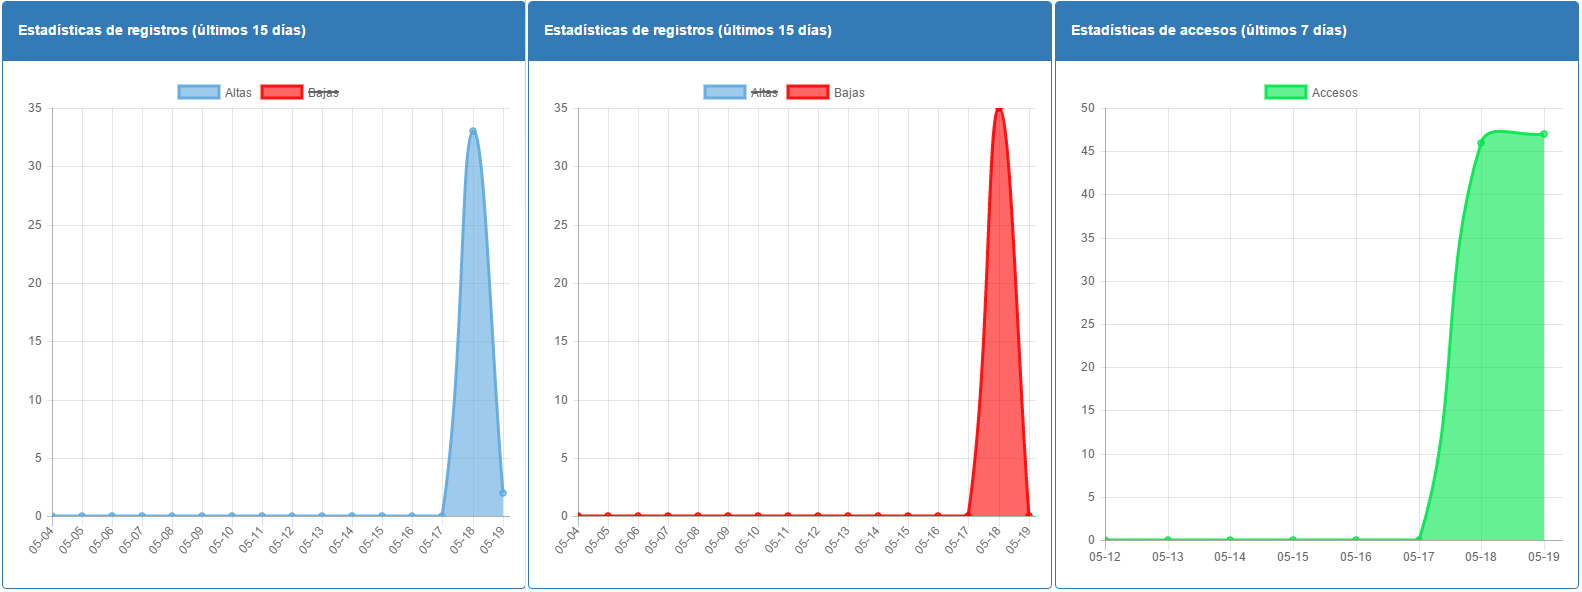
\includegraphics[width=1\linewidth]{img/altas-bajas-accesos}
				\caption{Registros, cuentas borradas en la aplicación en los útlimos 15 días y accesos de los usuarios (no únicos) a la apliación en los últimos 7 días.}
				\label{fig:altas-bajas-accesos}
			\end{figure}
			
			\begin{figure}[H]
				\centering
				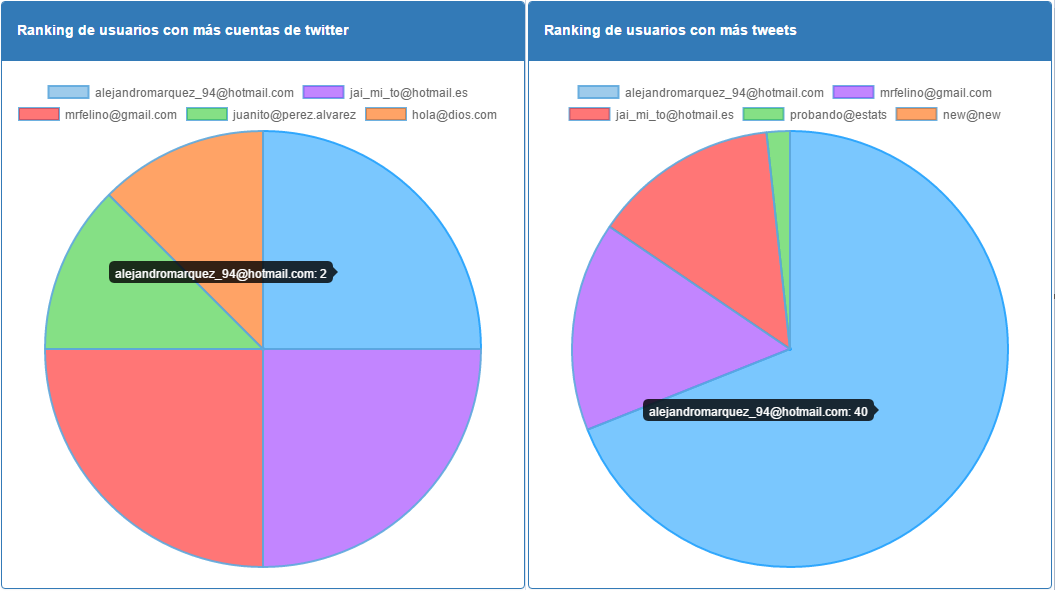
\includegraphics[width=1\linewidth]{img/rankingsAdmin}
				\caption{Ranking de cuentas con mayor número de tweets enviados (izquierda) y ranking de cuentas de la aplicación con mayor número de cuentas de twitter asociadas cada una (derecha).}
				\label{fig:rankingsAdmin}
			\end{figure}
	
	\subsection{Analíticas de usuario} 

		\paragraph{} El interés de estas gráficas para el usuario reside en informarle de la diferente repercursión que tienen sus disintas cuentas de \textit{Twitter} asociadas. 
		
			\begin{figure}[H]
				\centering
				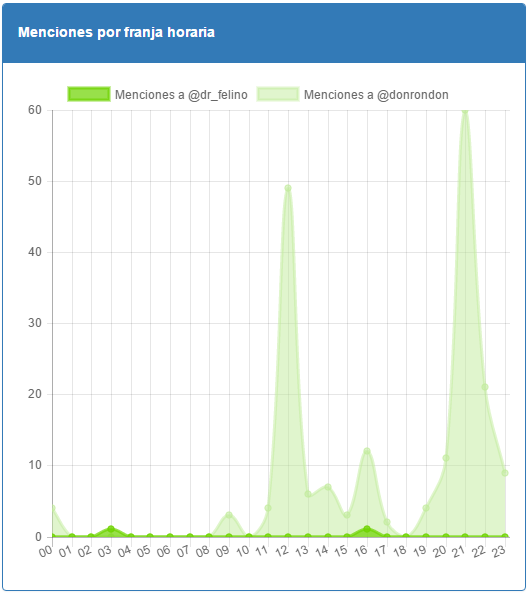
\includegraphics[width=0.6\linewidth]{img/mencionesHoras}
				\caption{Número de menciones con cada cuenta del usuario distribuidas por franja horaria.}
				\label{fig:mencionesHoras}
			\end{figure}
			
			\begin{figure}[H]
				\centering
				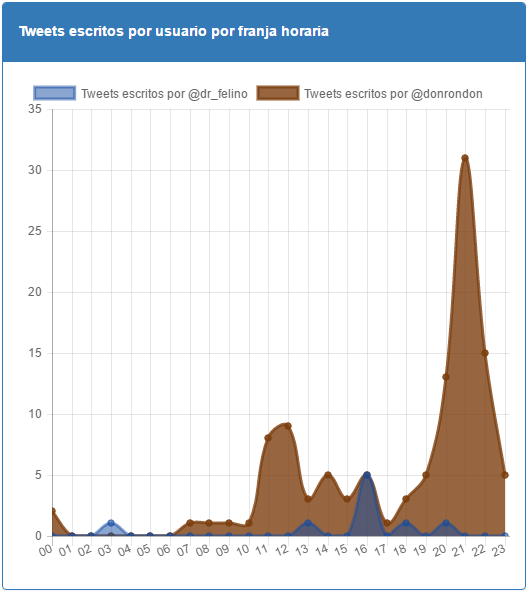
\includegraphics[width=0.6\linewidth]{img/tweetsHoras}
				\caption{Número de tweets enviados con cada cuenta del usuario distribuidos por franja horaria.}
				\label{fig:tweetsHoras}
			\end{figure}
			
			\begin{figure}[H]
				\centering
				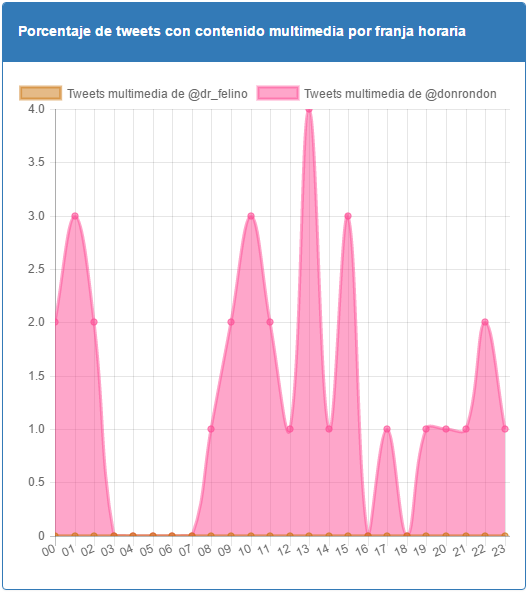
\includegraphics[width=0.6\linewidth]{img/tweetsMultimedia}
				\caption{Porcentaje de tweets con contenido multimedia con cada cuenta del usuario y distribuidos por franja horaria.}
				\label{fig:tweetsMultimedia}
			\end{figure}
			
			\begin{figure}[H]
				\centering
				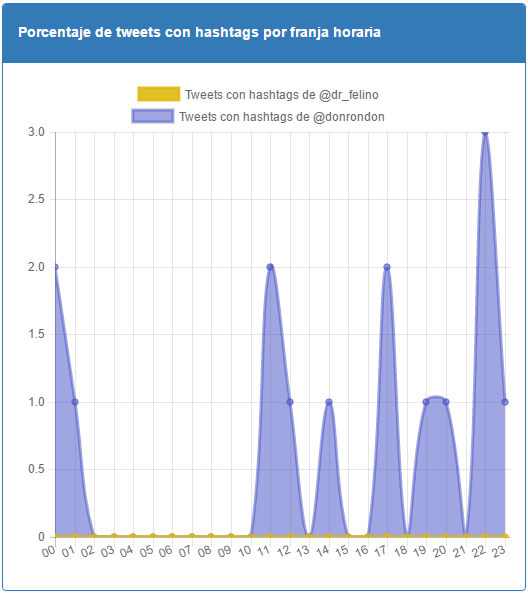
\includegraphics[width=0.6\linewidth]{img/hashtagsHoras}
				\caption{Porcentaje de tweets con contenido multimedia con cada cuenta del usuario y distribuidos por franja horaria.}
				\label{fig:hashtagsHoras}
			\end{figure}
			
			\begin{figure}[H]
				\centering
				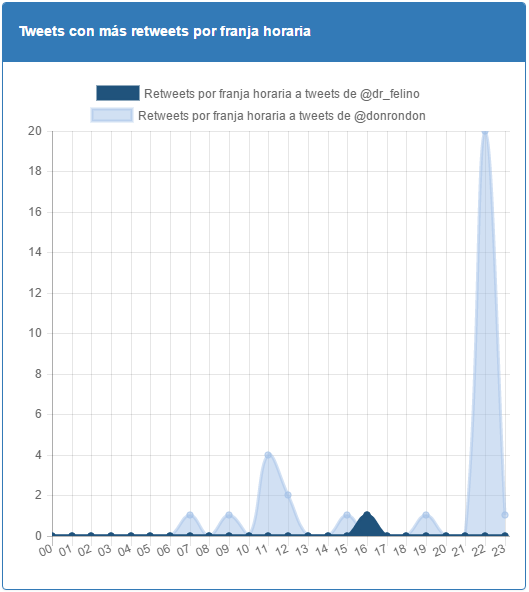
\includegraphics[width=0.6\linewidth]{img/retweetsHoras}
				\caption{Cantidad de retweets realizados sobre tweets escritos en determinada franja horaria para cada cuenta del usuario.}
				\label{fig:retweetsHoras}
			\end{figure}
			
			\begin{figure}[H]
				\centering
				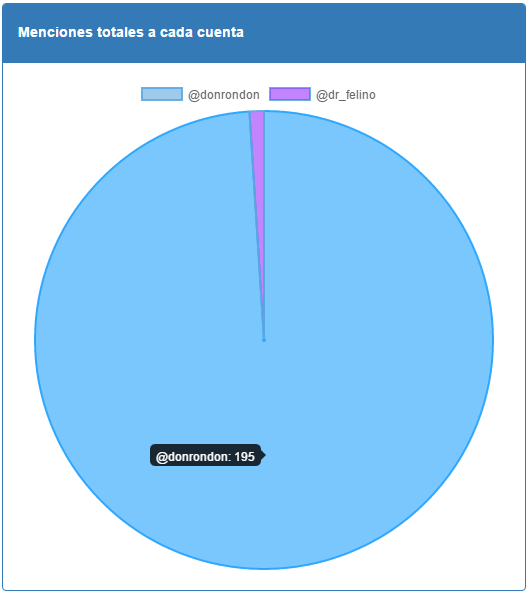
\includegraphics[width=0.6\linewidth]{img/mencionesCuentas}
				\caption{Cantidad de menciones para cada cuenta del usuario (representa impacto de cada cuenta de twitter en su entorno.)}
				\label{fig:mencionesCuentas}
			\end{figure}

\section{Implementación}

	\paragraph{} Para el desarrollo de la aplicación web propuesta se ha hecho uso del conjunto de tecnologías denominado como \textbf{\textit{MEAN Stack}} (\textit{MongoDB}, \textit{Express}, \textit{AngularJS}, \textit{Node}). Para el desarrollo del \textit{front-end} se han usado \textit{AngularJS + Bootstrap} y para el desarrollo del \textit{back-end} se han utilizado \textit{MongoDB} para la base de datos y \textit{Express} y \textit{Node} para el desarrollo del servidor, lo cual asegura escalabilidad.

	\subsection{Desarrollo de \textit{front-end}}
	
		\paragraph{} Se ha optado por realizar la gestión de enrutamiento mediante \textit{AngularJS} aprovechando las facilidades que proporciona en la implementación de un modelo vista-controlador.
		
		\paragraph{} En primer lugar, se ha definido en un fichero \textbf{public/app.js} el conjunto de estados (vistas) en los que se puede encontrar la aplicación de forma, que es el que se encarga de redirigir correctamente cualquier petición de cambio de estado. Éste módulo también se encarga de asignar a cada estado una vista \textit{.html} con un controlador \textit{.js}.
	
		\paragraph{} Cada controlador gestiona de forma dinámica su vista asociada. En el caso de invocar a un \textit{API} externa se comunica con el módulo principal de los controladores (\textit{public/app.js}) y es éste el único que realiza las peticiones \textbf{.http}. Así se consige modular el código, de forma que es más fácil su depuración.
	
		\paragraph{} Por último, todas las vistas (\textit{.html}) utilizan \textit{Bootstrap} para asegurar que la aplicación se pueda visualizar correctamente en dispositivos con pantallas de distintos tamaños.
		
	\subsection{Desarrollo de \textit{back-end}}
	
		\paragraph{} Dado que es el \textit{front-end} el que se encarga de enrutar las peticiones, la función del servidor en este aspecto es la de para cualquier petición que reciba redirigir al \textit{front-end}. De esta forma el servidor se limita a proporcionar los distintos servicios web propuestos (\textit{control de usuarios}, \textit{acortador de URLs} y servicio de \textit{estadísticas}).
		
		\paragraph{} El servidor se ha implementado con \textit{node.js}, de esta forma se asegura una buena escalabilidad de la aplicación. En este sentido la gestión de la base de datos mediante \textit{Mongoose} también ayuda a mejorar esta característica.
		
\section{Modelo de navegación}
\paragraph{}A continuación se muestran capturas de pantalla de la aplicación con una breve descripción de los enlaces existentes entre dichas pantallas.
\begin{figure}[H]
	\centering
	
\includegraphics[width=350px]{img/main.png}
	\caption{Vista principal de la aplicación}
	\label{fig:diagarq}
\end{figure}
\paragraph{} Desde esta vista, \textbf{principal}, se puede acceder a:
\begin{itemize}
	\item La vista de login, a través del botón Entrar
	\item La vista de registro, a través del botón Registrarse
\end{itemize}
\begin{figure}[H]
	\centering
	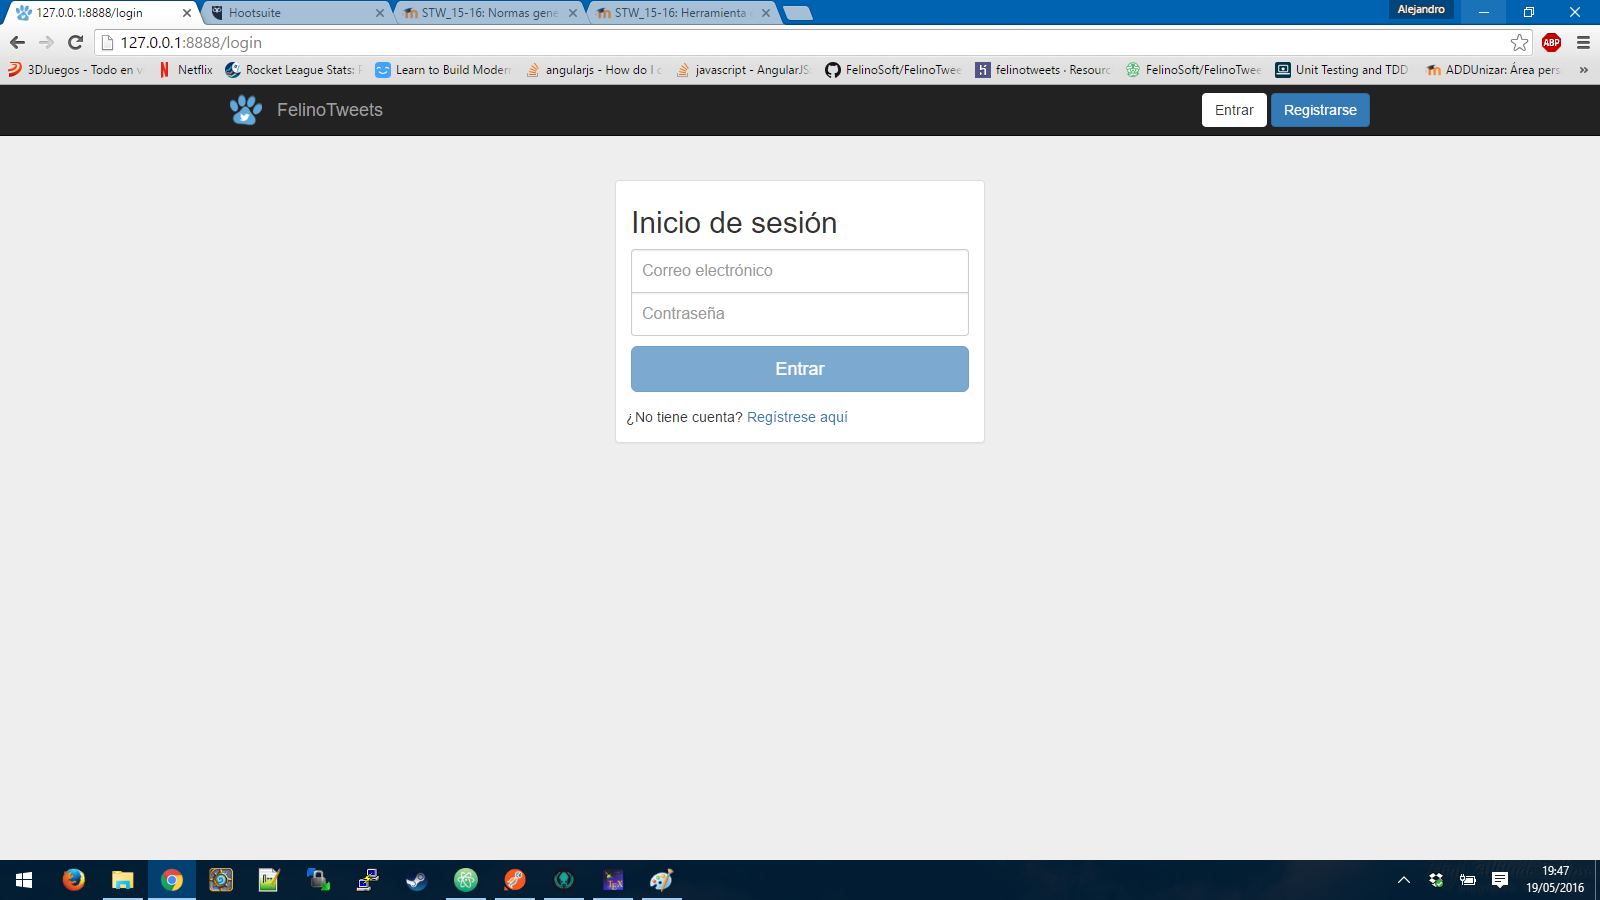
\includegraphics[width=350px]{img/login.png}
	\caption{Vista de login de la aplicación}
	\label{fig:diagarq}
\end{figure}
\paragraph{} Desde esta vista, \textbf{login}, se puede acceder a:
\begin{itemize}
	\item La vista de login, a través del botón Entrar
	\item La vista de registro, a través del botón Registrarse
	\item La vista de home, a través de un correcto login en la aplicación
	\item La vista del panel de administrador, a través de un correcto login del administrador en la aplicación
\end{itemize}
\begin{figure}[H]
	\centering
	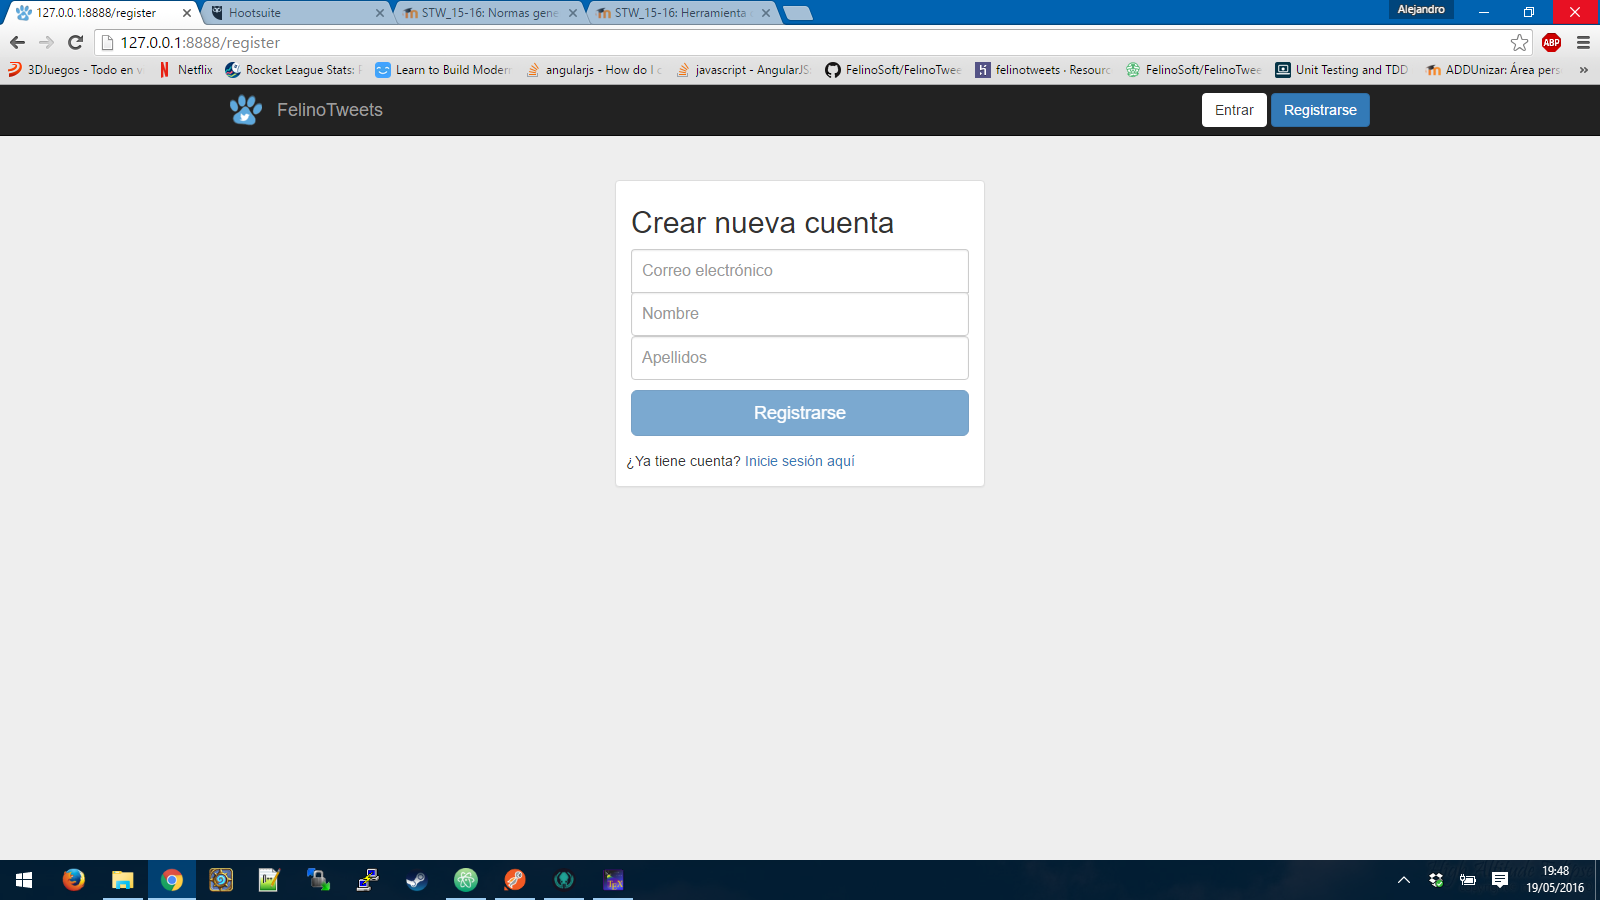
\includegraphics[width=350px]{img/register.png}
	\caption{Vista de registro de la aplicación}
	\label{fig:diagarq}
\end{figure}
\paragraph{} Desde esta vista, \textbf{registro}, se puede acceder a:
\begin{itemize}
	\item La vista de login, a través del botón Entrar
	\item La vista de registro, a través del botón Registrarse
	\item La vista de home, a través de un correcto registro en la aplicación
\end{itemize}
\begin{figure}[H]
	\centering
	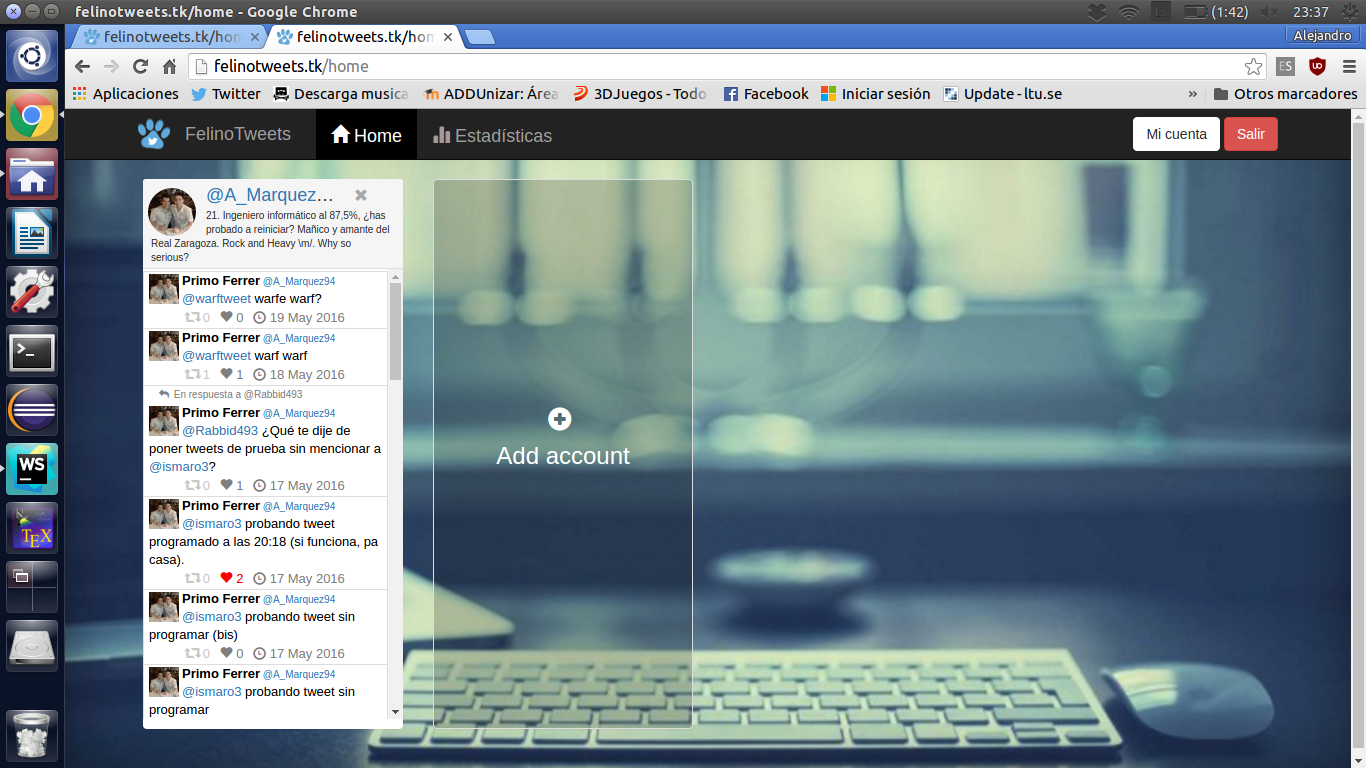
\includegraphics[width=350px]{img/home-twitter.png}
	\caption{Vista de home de la aplicación}
	\label{fig:diagarq}
\end{figure}
\paragraph{} Desde esta vista, \textbf{home}, se puede acceder a:
\begin{itemize}
	\item La vista de perfil, a través del botón Mi cuenta
	\item La vista principal, a través del botón Salir
	\item La vista de la cuenta de twitter, a través de los enlaces situados en los nombres de las cuentas de twitter que haya
	\item La vista de estadísticas del usuario, a través del botón Estadísticas
	\item La vista de autorizar cuenta de twitter, a través del botón Add account
\end{itemize}
\begin{figure}[H]
	\centering
	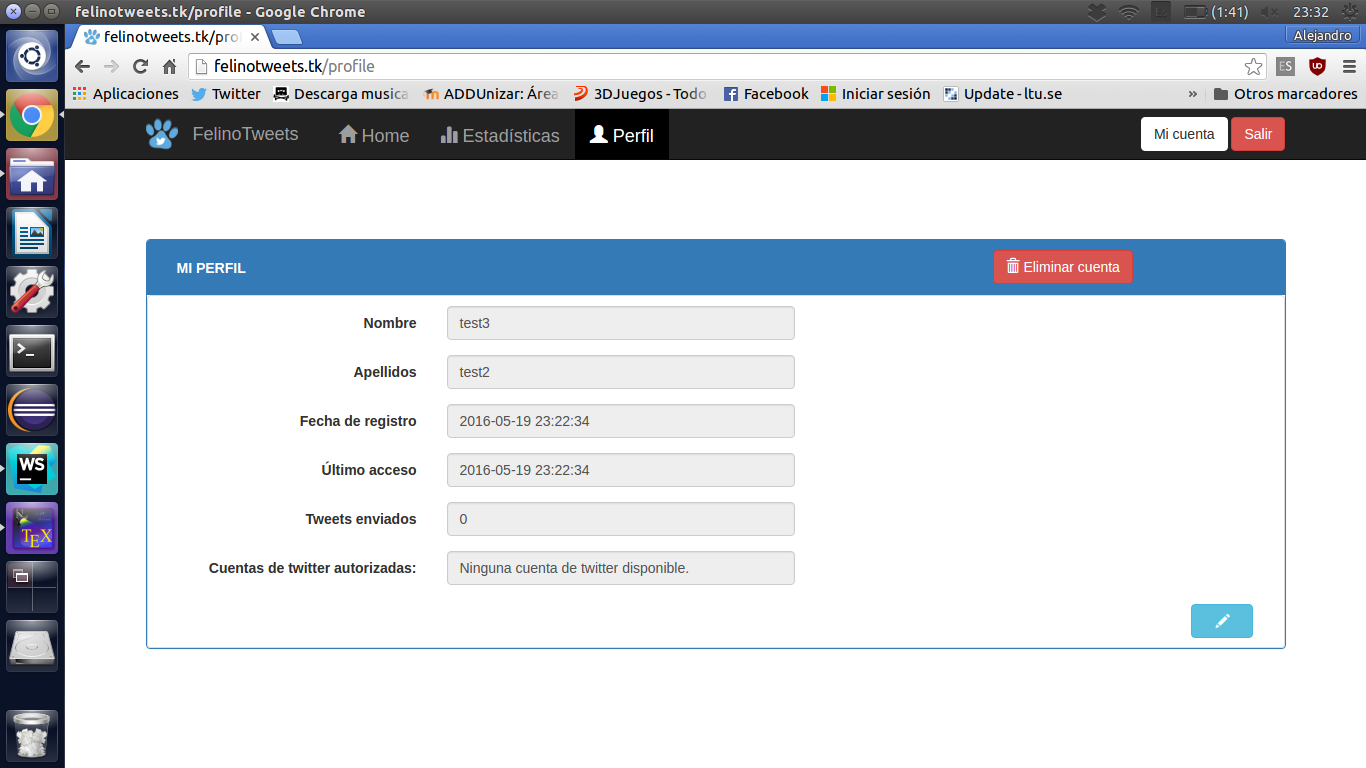
\includegraphics[width=350px]{img/profile.png}
	\caption{Vista de perfil de la aplicación}
	\label{fig:diagarq}
\end{figure}
\paragraph{} Desde esta vista, \textbf{perfil}, se puede acceder a:
\begin{itemize}
	\item La vista de perfil, a través del botón Mi cuenta
	\item La vista principal, a través del botón Salir
	\item La vista de home, a través del botón Home
	\item La vista de estadísticas del usuario, a través del botón Estadísticas
\end{itemize}
\begin{figure}[H]
	\centering
	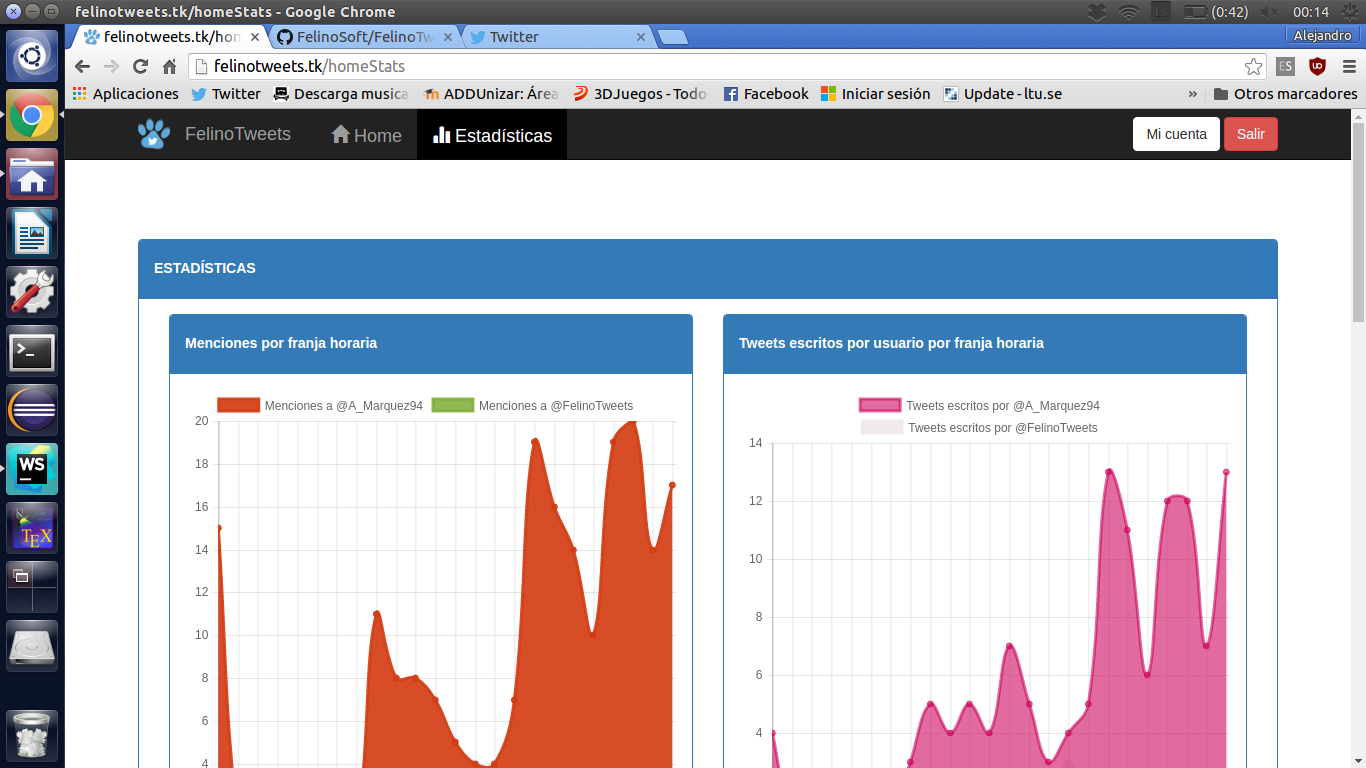
\includegraphics[width=350px]{img/estadisticas.png}
	\caption{Vista de estadísticas de la aplicación}
	\label{fig:diagarq}
\end{figure}
\paragraph{} Desde esta vista, \textbf{estadisticas}, se puede acceder a:
\begin{itemize}
	\item La vista de perfil, a través del botón Mi cuenta
	\item La vista principal, a través del botón Salir
	\item La vista de home, a través del botón Home
\end{itemize}
\begin{figure}[H]
	\centering
	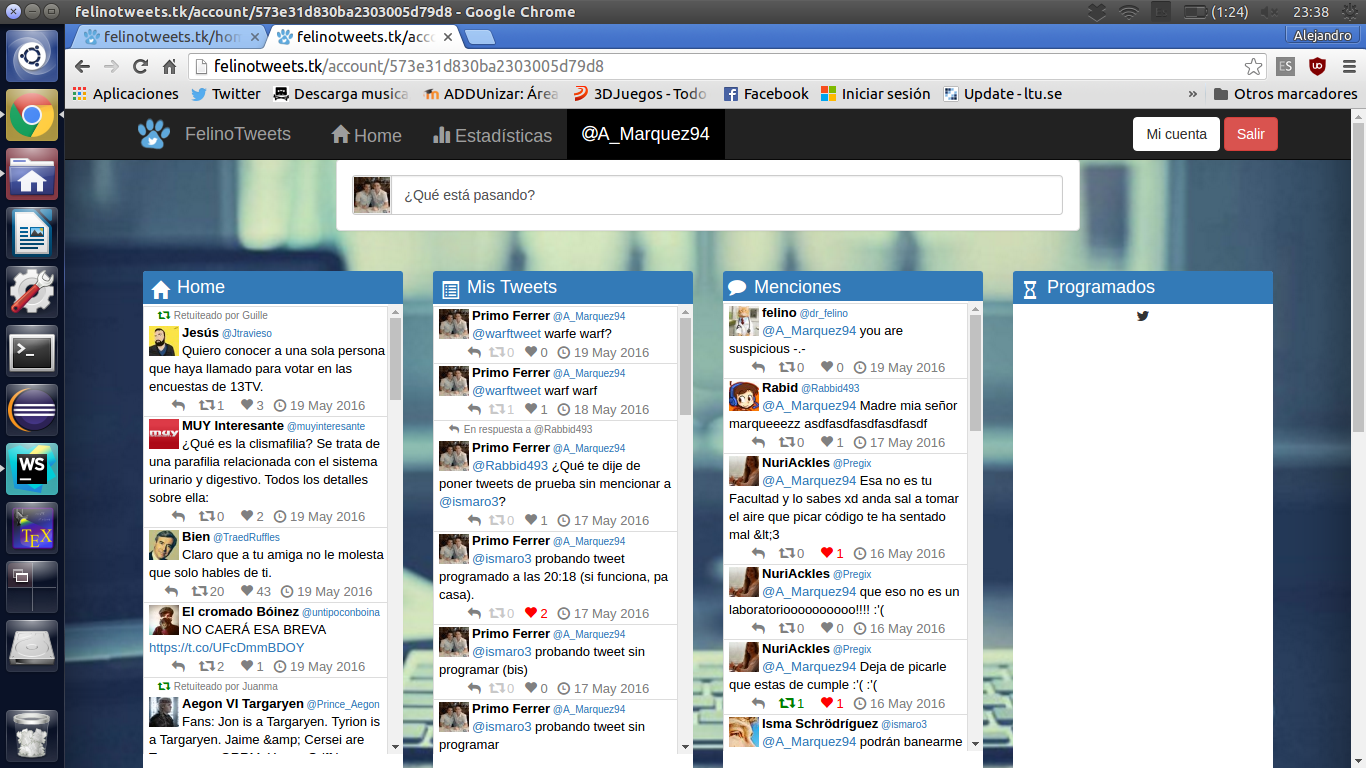
\includegraphics[width=350px]{img/account.png}
	\caption{Vista de la cuenta de twitter de la aplicación}
	\label{fig:diagarq}
\end{figure}
\paragraph{} Desde esta vista, \textbf{cuenta de twitter}, se puede acceder a:
\begin{itemize}
	\item La vista de perfil, a través del botón Mi cuenta
	\item La vista principal, a través del botón Salir
	\item La vista del home, a través del botón Home
	\item La vista de estadísticas del usuario, a través del botón Estadísticas
\end{itemize}
\begin{figure}[H]
	\centering
	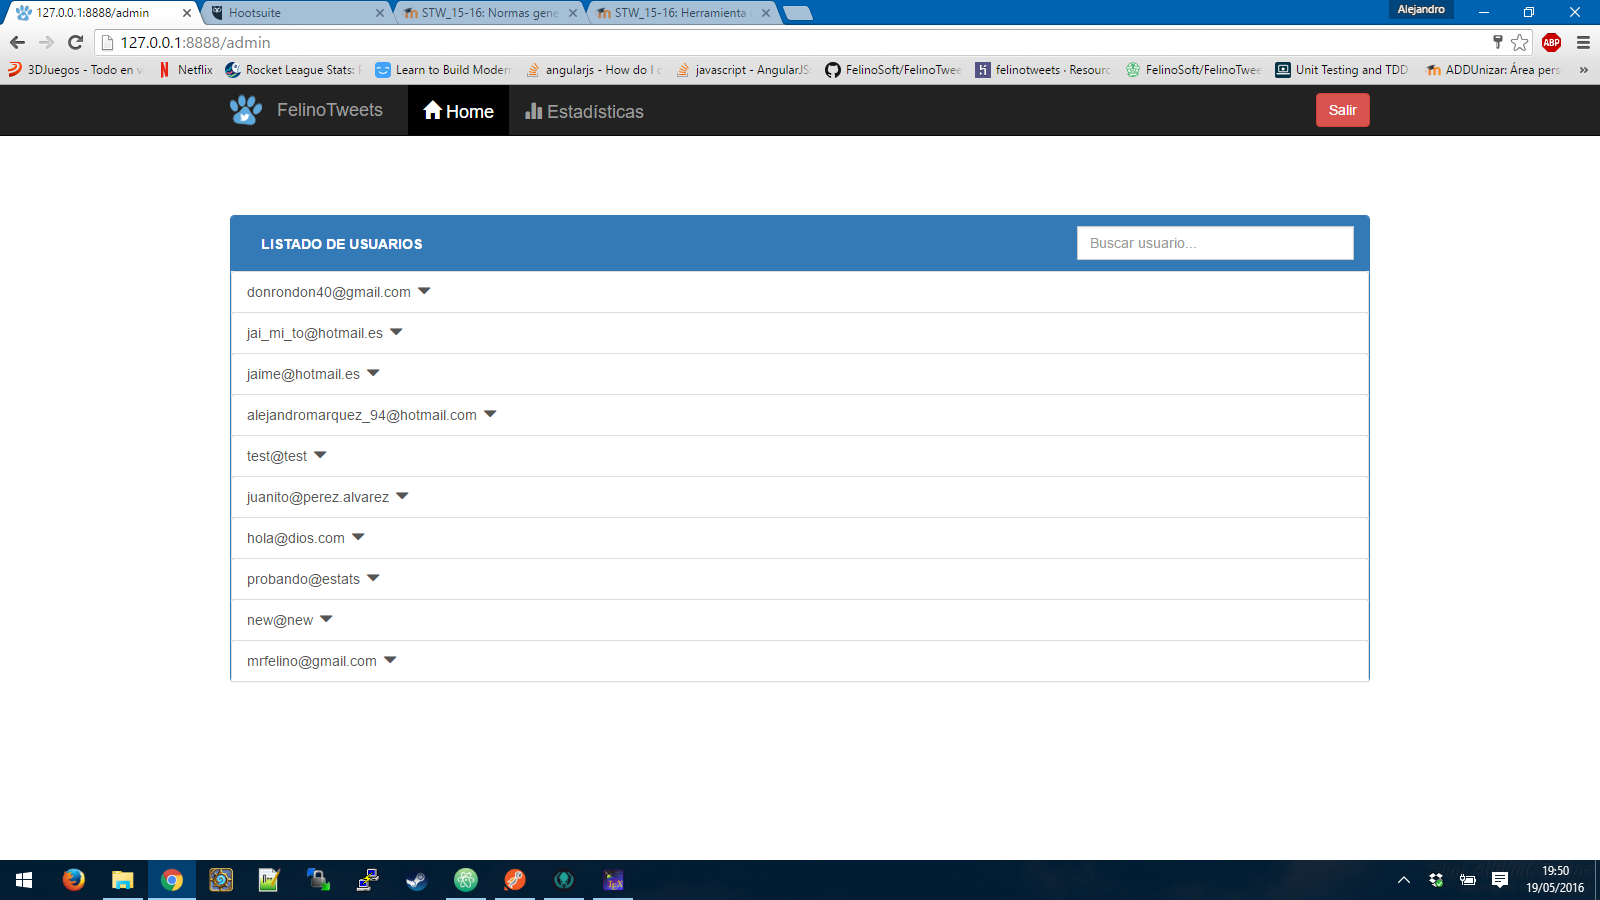
\includegraphics[width=350px]{img/admin.png}
	\caption{Vista del panel del administrador de la aplicación}
	\label{fig:diagarq}
\end{figure}
\paragraph{} Desde esta vista, \textbf{el panel del administrador}, se puede acceder a:
\begin{itemize}
	\item La vista principal, a través del botón Salir
	\item La vista de estadísticas del administrador, a través del botón Estadísticas
\end{itemize}
\begin{figure}[H]
	\centering
	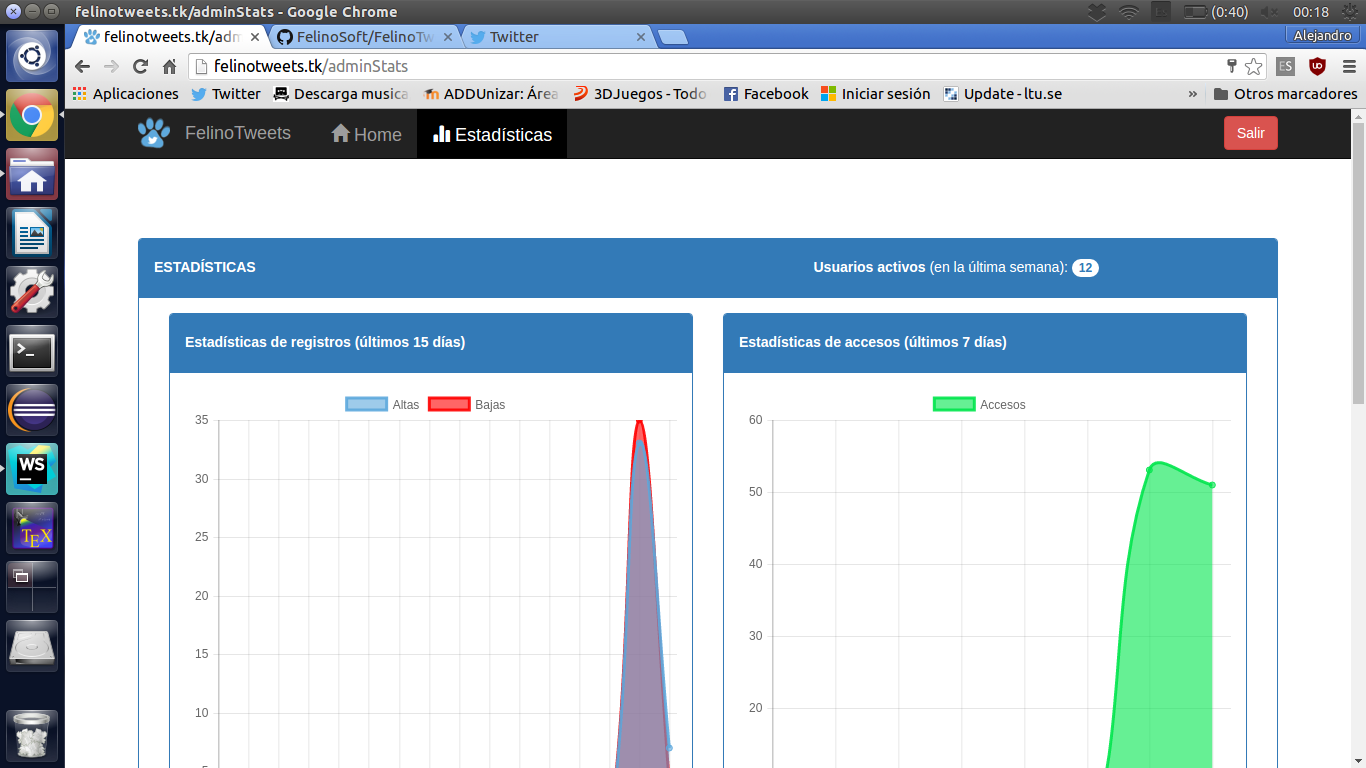
\includegraphics[width=350px]{img/estadisticasadmin.png}
	\caption{Vista de las estadísticas del administrador de la aplicación}
	\label{fig:diagarq}
\end{figure}
\paragraph{} Desde esta vista, \textbf{estadísticas del administrador}, se puede acceder a:
\begin{itemize}
	\item La vista principal, a través del botón Salir
	\item La vista del panel del administrador, a través del botón Home
\end{itemize}
\section{Despliegue del sistema (instrucciones)}
\paragraph{}Para desplegar el sistema se hace uso de Heroku, una plataforma que permite montar la aplicación de manera gratuita (con limitaciones, pero para el alcance del proyecto es más que suficiente) de una manera fácil y sencilla. Está configurado de tal manera que se despliegue automáticamente a partir del repositorio de GitHub de \href{https://github.com/FelinoSoft/FelinoTweets}{FelinoTweets}. De esta forma, la aplicación se actualizará con cada commit realizado sobre la branch principal del repositorio.
\paragraph{}La aplicación contiene un fichero de configuración, siguiendo la ruta a partir de la raíz \textit{/confi/config.json}. En él hay que definir los siguientes campos;
\begin{itemize}
\item \textbf{domain}: el dominio de la aplicación.
\item \textbf{port}: el puerto en el que escuchará la aplicación.
\item \textbf{consumerKey}: la clave de consumidor de Twitter, para realizar las operaciones con el API de Twitter (esto se explicará más adelante).
\item \textbf{consumerSecret}: la clave secreta de Twitter, que junto con la anterior, permite autentificarse como una App de Twitter.
\item \textbf{databaseAddress}: dirección de la base de datos sobre la que se realizarán las consultas y almacenarán los datos de la aplicación.
\item \textbf{API}: ruta de la API de la aplicación, sobre la que se situarán los endpoints.
\end{itemize}

\paragraph{}Los apartados \textit{consumerKey} y \textit{consumerSecret} contienen las claves de la aplicación de Twitter. Para poder realizar operaciones al API de Twitter, es necesario haber creado antes una Twitter App, en su página oficial, que permitirá a los usuarios autentificarse o loguearse a Twitter a través de la aplicación, y de esta manera realizar en su lugar operaciones (como postear tweets, hacer búsquedas...). Estas dos claves sirven para identificarse de una manera segura como aplicación de Twitter, y no deben ser ni compartidas ni públicas.

\paragraph{}La base de datos de la aplicación está proporcionada por \href{https://mlab.com/}{mLab}, un servicio de base de datos \textit{Database-as-a-Service} para MongoDb. Al igual que Heroku, tiene ciertas limitaciones, pero sus funcionalidades son más que suficientes para el proyecto.

\paragraph{}Por último, para terminar de desplegar el sistema y dejarlo listo para funcionar, hay que añadir un usuario que actuará como administrador, y de esta manera, podrá realizar operaciones sobre los usuarios y sus cuentas.

\section{Validación (test, pruebas realizadas)}
\paragraph{}Para probar el correcto funcionamiento de la aplicación, se han ido probando mediante Postman todas las operaciones disponibles sobre los endpoints de las APIs, obteniendo el comportamiento deseado. Finalmente, se ha realizado un recorrido por toda la aplicación, que se detalla a continuación:
\begin{itemize}
	\item \textbf{Paso: }Registro de un usuario. \textbf{Resultado:} Usuario registrado correctamente. Redirigido a home.
	\item \textbf{Paso: }Editar un usuario. \textbf{Resultado: }Datos editados correctamente. Se actualizan inmediatamente.
	\item \textbf{Paso: }Cerrar sesión. \textbf{Resultado: }Redirigido a pantalla principal.
	\item \textbf{Paso: }Loguear con los nuevos datos. \textbf{Resultado: }Entra correctamente.
	\item \textbf{Paso: }Añadir nueva cuenta de twitter. \textbf{Resultado: }Cuenta agregada correctamente.
	\item \textbf{Paso: }Entrar en la cuenta de twitter. \textbf{Resultado: }Entra correctamente.
	\item \textbf{Paso: }Añadir un hastag. \textbf{Resultado: }Hashtag añadido correctamente.
	\item \textbf{Paso: }Enviar un tweet \textbf{Resultado: }Tweet enviado correctamente.
	\item \textbf{Paso: }Dar un fav \textbf{Resultado: }Fav realizado correctamente.
    \item \textbf{Paso: }Dar un retweet. \textbf{Resultado: }Retweet realizado correctamente.
    \item \textbf{Paso: }Programar un tweet. \textbf{Resultado: }Tweet programado correctamente.
    \item \textbf{Paso: }Esperar el envío del tweet programado. \textbf{Resultado: }Envío realizado correctamente.
    \item \textbf{Paso: }Programar otro tweet y eliminarlo. \textbf{Resultado: }Tweet programado y eliminado correctamente.
    \item \textbf{Paso: }Añadir otro hashtag y eliminarlo. \textbf{Resultado: }Hashtag añadido y eliminado correctamente.
    \item \textbf{Paso: }Añadir otra cuenta de twitter y ver estadísticas. \textbf{Resultado: }Se observan las estadísticas del usuario correctamente.
    \item \textbf{Paso: }Eliminar una cuenta de Twitter. \textbf{Resultado: }Cuenta de Twitter eliminada correctamente.
    \item \textbf{Paso: }Salir sesión y registrarse con otra cuenta, para después entrar con la de administrador. \textbf{Resultado: }Pantalla del administrador mostrada correctamente (se observa el listado de todos los usuarios).
    \item \textbf{Paso: }Ver info de un usuario, desplegarla, y editarla. \textbf{Resultado: }Información mostrada y editada correctamente.
    \item \textbf{Paso: }Ver estadísticas del administrador. \textbf{Resultado: }Estadísticas mostradas correctamente.
    \item \textbf{Paso: }Eliminar un usuario desde la pantalla de admin. \textbf{Resultado: }Usuario eliminado correctamente.
    \item \textbf{Paso: }Iniciar sesión como el usuario borrado. \textbf{Resultado: }Error al entrar.
    \item \textbf{Paso: }Iniciar sesión como el usuario antes creado, y borrar su cuenta. \textbf{Resultado: }Cuenta eliminada correctamente.
    \item \textbf{Paso: }Entrar con el móvil. \textbf{Resultado: }La aplicación es responsive.
\end{itemize}

\section{Análisis de problemas}

	\paragraph{} Dado que es la primera vez que el equipo afronta un desarrollo web de estas características, se ha encontrado como princpal dificultad el aprendizaje de las nuevas tecnologías con las que se requería realizar el proyecto.
	
	\paragraph{} Por otro lado, ha resultado complicado plantear la estructura del código a implementar en cuanto a cómo debía gestionarse el enrutamiento y cual es la mejor estrategia para organizar los directorios de una aplicación con características como múltiples vistas y de las dimensiones que tiene la aplicación propuesta. Todas estas cuestiones cobran mayor importancia al ser la primera vez que se afrontan.

\section{Conclusiones}
	\subsection{Conclusiones del proyecto}
	
		\paragraph{} La realización de este proyecto ha generado como resultado una aplicación web \textit{responsive} que permite al usuario gestionar cuentas de \textit{Twitter} así como ver estadísticas de las mismas.
		
		\paragraph{} Durante el desarrollo del proyecto se ha trabajo con un \textit{API} externa que es la de \textit{Twitter}, lo cual ha resultado útil a la hora de entender cómo se comunican las aplicaciones web actualmente. 
	
	\subsection{Valoración personal del grupo}
	
		\paragraph{} El proyecto ha ayudado principalmente a comprender el funcionamiento de un servicio web y de los canales de comunicación así como tecnologías mas usadas actualmente, lo cual puede servir de ayuda para futuros desarrollos.
	
		\paragraph{} El desarrollo con nuevas tecnologías ha sido desafiante pero al mismo tiempo gratificante, ya que se obtienen resultados simples con rapidez. El equipo ha quedado satisfecho con el resultado conseguido aunque se considera que el tiempo disponible para realizarlo ha sido muy ajustado.
		
	\subsection{Valoración personal de cada miembro}
	
	
		\subsubsection{Alejandro Márquez}
		
			\paragraph{}Considero que el proyecto en sí (y la asignatura en general) ha sido muy provechoso, puesto que las tecnologías empleadas están muy de actualidad, y resulta muy interesante trabajar con ellas. Además, con el proyecto he aprendido un poco a manejarlas, y me he quedado con ganas de seguir trabando en él para ampliarlo.

			\paragraph{}Como puntos en contra, he visto el curso muy descompensado, empezando muy despacio y sin nada de trabajo, y acumulándose este proyecto para las últimas semanas, que junto con las rectas finales de los demás cursos, se ha hecho muy cuesta arriba, y por lo tanto, no ha dado tiempo a dedicarle toda la atención y detalle que me habría gustado. Además, si bien con las prácticas he aprendido a usar las distintas tecnologías, me he sentido perdido a la hora de establecer la estructura de un proyecto ''grande'' como es este, sin saber muy bien como organizarlo. He echado de menos algo de guía en ese sentido.

			\paragraph{}Como conclusión del proyecto y de la asignatura, pese al detalle del tiempo, que creo que se podría solucionar distribuyéndolo un poco mejor (empezar antes las prácticas y dar antes la información del trabajo), esta ha sido sin duda la asignatura más interesante y provechosa del cuatrimestre.
		
		\subsubsection{Jaime Ruiz-Borau}
			
			\paragraph{} Ha sido uno de los trabajos de los cuales puedo decir que me siento más orgulloso por el resultado que ha dado. Aunque nos costó al principio finalmente hemos conseguido una simpática aplicación que interacciona correctamente con el API de Twitter y que se parece bastante a otras soluciones como la que se planteó en el enunciado.
			
			\paragraph{}Quizás lo más complicado del trabajo para mi ha sido la parte del front end y el diseño en general de la web, nos ha traído muchos más quebraderos de cabeza que el back end. También hacia el final nos ha faltado un poco de tiempo para retocar y mejorar todas las cosas que teníamos en mente.
		
		\subsubsection{Alejandro Royo}
		
			\paragraph{} El desarrollo del trabajo me ha resultado gratificante por un lado por las tecnologías usadas que no conocía y también por la utilidad que se aprecia al realizar este tipo de aplicaciones. De todas formas, creo que el tiempo proporcionado para realizar el trabajo ha sido más bien escaso.
			
			\paragraph{} Como posible solución al poco tiempo que he percibido creo que igual sería mejor integrarlo más con las prácticas en el sentido de permitir que se vaya integrando cada práctica en el trabajo desde el principio.
	
\end{document}